\documentclass{beamer}
\usetheme{Madrid}
\usecolortheme{default}

\usepackage{amsmath, amssymb}
\usepackage{mathtools}
\usepackage{graphicx}
\usepackage{tikz}
\usetikzlibrary{fit, positioning, shapes.geometric}
\usepackage{booktabs} % Added for table styling
\usetikzlibrary{fit, decorations.pathreplacing}
\usetikzlibrary{overlay-beamer-styles}



\newcommand{\Parcurly}[1]{\left\{ #1 \right\}}
\newcommand{\parcurly}[1]{\{ #1 \}}
\newcommand{\bparcurly}[1]{\bigl\{ #1 \bigr\}}
\newcommand{\bbparcurly}[1]{\Bigl\{ #1 \Bigr\}}

\newcommand{\Parround}[1]{\left( #1 \right)}
\newcommand{\parround}[1]{( #1 )}
\newcommand{\bparround}[1]{\bigl( #1 \bigr)}
\newcommand{\bbparround}[1]{\Bigl( #1 \Bigr)}

\newcommand{\Parsquared}[1]{\left[ #1 \right]}
\newcommand{\parsquared}[1]{[ #1 ]}
\newcommand{\bparsquared}[1]{\bigl[ #1 \bigr]}

\newcommand{\Parstraight}[1]{\left| #1 \right|}
\newcommand{\parstraight}[1]{| #1 |}
\newcommand{\bparstraight}[1]{\bigl| #1 \bigr|}

\newcommand{\Partriangle}[1]{\left< #1 \right>}
\newcommand{\partriangle}[1]{< #1 >}




\title[Regularity for Stable Graphs]{The Regularity Lemma for Stable Graphs and its Applications in Property Testing}
\author{Severino Da Dalt}
\institute{Supervised by Lluís Vena Cros}
\date{\today}

\begin{document}

% Title page
\begin{frame}
    \titlepage
\end{frame}

% ---
% Table of contents
\begin{frame}{Table of contents}
    \begin{enumerate}
        \item Introduction to Szemerédi's Regularity Lemma
        \item Stable Graphs and the Stable Regularity Lemma
        \item Sketch of the Proof of the Stable Regularity Lemma
        \item Property Testing of $H$-freeness in Stable Graphs
        \item Conclusion and Future Work
    \end{enumerate}
\end{frame}

% ---
% Regularity
\begin{frame}{Introduction to Szemerédi's Regularity Lemma}
    The idea of the SzRL is that all graphs can be partitioned in such a way that most pairs of parts
    behave in a quasi-random way, a property which is formalized as \emph{regularity}.

    \begin{definition}
        Given $\epsilon > 0$ and a graph $G$, a pair of (not necessarily disjoint) subsets of vertices $A, B \subseteq G$
        is said to be \emph{$\epsilon$-regular} if for all $A' \subseteq A$ and $B' \subseteq B$ such that
        $|A'| \geq \epsilon |A|$ and $|B'| \geq \epsilon |B|$, we have
        \[
            |d(A', B') - d(A, B)| \leq \epsilon.
        \]
    \end{definition}
\end{frame}

% Regular partitions
\begin{frame}{Introduction to Szemerédi's Regularity Lemma}
    When most of the pairs satisfy this property, we say that the partition is \emph{regular}.

    \begin{definition}
        Let $G$ be a graph and let $\epsilon > 0$.
        An \emph{$\epsilon$-regular partition} of $G$ is a partition of its vertex set into $k$ parts
        $\parcurly{A_1, \ldots, A_k}$ with remainder set $B$ such that:
        \begin{itemize}
            \item $|B| \leq \epsilon |G|$, and may be empty.
            \item All but at most $\epsilon k^2$ of the pairs $(A_i, A_j)$ with $1 \leq i < j \leq k$ are
                $\epsilon$-regular.
        \end{itemize}
    \end{definition}
\end{frame}

% SzRL
\begin{frame}{Introduction to Szemerédi's Regularity Lemma}
    \begin{theorem}[Szemerédi's Regularity Lemma, \cite{regular_partitions_of_graphs}]
        For every $\epsilon > 0$ and every positive integer $m$, there exists a positive integer $M = M(\epsilon, m)$
        such that every graph with at least $m$ vertices admits an $\epsilon$-regular partition
        $\parcurly{A_1, \ldots, A_k}$ and remainder $B$ with $m \leq k \leq M$, with $|A_1| = \dots = |A_k|$.
    \end{theorem}

    Crucially, the theorem proves that the number of parts $k$ does not grow with the size of the graph,
    but only depends on $\epsilon$ (and $m$).
    % The SzRL sees extensive use in combinatorics, number theory, and computer science.
\end{frame}

% Limitations of SzRL
\begin{frame}{Introduction to Szemerédi's Regularity Lemma}
    However, the lemma has two major drawbacks:
    \begin{enumerate}
        \item The bound on the number of parts $M$ is a \emph{tower-type} function of $\epsilon$,
            i.e. a power-tower of height polynomial in $1/\epsilon$.
            This is unavoidable, as shown by Gowers~\cite{gowers_lower_bound}.
        \item The partition may contain some irregular pairs.
            This is also unavoidable, and the half-graph $H_n$ is an example.
    \end{enumerate}
\end{frame}

% ---

% half-graph
\begin{frame}{Stable Graphs and the Stable Regularity Lemma}
    \emph{Stable} graphs are those that do not contain a \emph{half-graph} as a bi-induced subgraph.
    \input{pictures/half-graph_presentation}
\end{frame}

% non-k-order property
\begin{frame}{Stable Graphs and the Stable Regularity Lemma}
    \begin{definition} \label{def:k_order_property}
        Let $G$ be a graph.
        We say that $G$ has the \emph{$k$-order property} if there exist two sequences of vertices
        $\Partriangle{a_i \mid i \in \parcurly{1, \dots, k}}$ and $\Partriangle{b_i \mid i \in \parcurly{1, \dots, k}}$ such that
        for all $i,j \leq k$, $a_i R b_j$ if and only if $i \geq j$.
        Otherwise, we say that $G$ has the \emph{non-$k$-order property} or that $G$ is \emph{$k$-stable}.
    \end{definition}

    The two sequences need not to be disjoint, and any combination of edges and non-edges may appear within
    the vertices of each sequence.
\end{frame}

% other non-k-orders
\begin{frame}{Stable Graphs and the Stable Regularity Lemma}
    \input{pictures/other_k-order_presentation}
\end{frame}

\begin{frame}{Stable Graphs and the Stable Regularity Lemma}
    \begin{theorem}[Stable Regularity Lemma,~\cite{regularity_lemmas_for_stable_graphs}] \label{thm:B}
        Each $k$-stable graph $G$ admits an equitable partition of its vertex set with at most
        ${c(k)\cdot(1/\epsilon)^{2^{k+1}}}$ parts such that ALL pairs of parts
        are $\epsilon$-regular and have density either less than $\epsilon$ or greater than $1 - \epsilon$.
    \end{theorem}

    Notably both limitations of the SzRL are overcome: the bound on the number of parts is
    polynomial in $1/\epsilon$, and there are no irregular pairs.
\end{frame}

% ---

% goodness and excellence
\begin{frame}{Sketch of the Proof of the Stable Regularity Lemma}
    \begin{definition}[Good,~\cite{regularity_lemmas_for_stable_graphs}] \label{def:epsilon_good}
        Let $G$ be a finite graph with the non-$k_*$-property.
        We say that $A \subseteq G$ is $\epsilon$-\emph{good} when for every $b \in G$ the truth value
        $t = t(b, A) \in \parcurly{0, 1}$ satisfies
        $\parstraight{\overline{B}_{A,b}} = \parstraight{\parcurly{a\in A \mid aRb \not\equiv t}} < \epsilon |A|$.
    \end{definition}

    \begin{definition}[Excellent,~\cite{regularity_lemmas_for_stable_graphs}] \label{def:epsilon_excellent}
        Let $G$ be a finite graph with the non-$k_*$-property.
        We say that $A \subseteq G$ is $(\epsilon, \zeta)$-\emph{excellent} when $A$ is $\epsilon$-good and, if $B$ is
        $\zeta$-good, then the truth value $t = t(B,A)$ satisfies $\parstraight{\parcurly{a \in A \mid t(a,B) \neq t(A,B)}} < \epsilon |A|$.
        In particular, we say $A$ is $\epsilon$-\emph{excellent} if $A$ is $(\epsilon, \epsilon)$-excellent.
    \end{definition}
\end{frame}

% example
\begin{frame}{Sketch of the Proof of the Stable Regularity Lemma}
    % 1
    \visible<1->{
        \input{pictures/non-monotonic_example_presentation}
    }
    % here explain:
    % - A is 1/5-good but B is not
    % - A is 1/5-excellent
    % - A is not 2/5-excellent, because B is 2/5-good but half of A has truth value 0 wrt B, and the other half 1
    % - this last fact also introduces a discrepancy in the original, as it is assumed that \epsilon-excellence is
    %   monotonic, which is not the case

    % 2
    \visible<2-> {\centering Do excellent subsets always exist?}
\end{frame}

% k-trees
\begin{frame}{Sketch of the Proof of the Stable Regularity Lemma}
    \begin{definition}[$k$-tree]<1-> \label{def:k-tree}
        A \emph{$k$-tree} in $G$ is an ordered pair $H = (\overline{c},\overline{b})$ comprising two (not necessarily
        disjoint) sequences:
        \begin{itemize}
            \item $\overline{c} = \parcurly{ c_\eta \in G \mid \eta \in \parcurly{0,1}^{<k} }$, the set of \emph{nodes} and
            \item $\overline{b} = \parcurly{ b_\rho \in G \mid \rho \in \parcurly{0,1}^k }$, the set of \emph{branches},
        \end{itemize}
        satisfying that for all $\eta \in \parcurly{0,1}^{<k}$ and $\rho \in \parcurly{0,1}^k$,
        if for some $\ell \in \parcurly{0, 1}$ we have $\eta \frown \Partriangle{\ell} \triangleleft \rho$, then
        $b_\rho R c_\eta \equiv \ell$.
    \end{definition}

    \begin{definition}[Tree bound]<2-> \label{def:tree_bound}
        Suppose $G$ is a finite graph.
        We denote the \emph{tree bound} $k_{**} = k_{**}(G)$ as the minimal positive integer such that there is no
        $k_{**}$-tree $H = (\overline{c},\overline{b})$ in $G$.
    \end{definition}
\end{frame}

% example of k-tree
\begin{frame}{Sketch of the Proof of the Stable Regularity Lemma}
    \begin{figure}
    \centering
    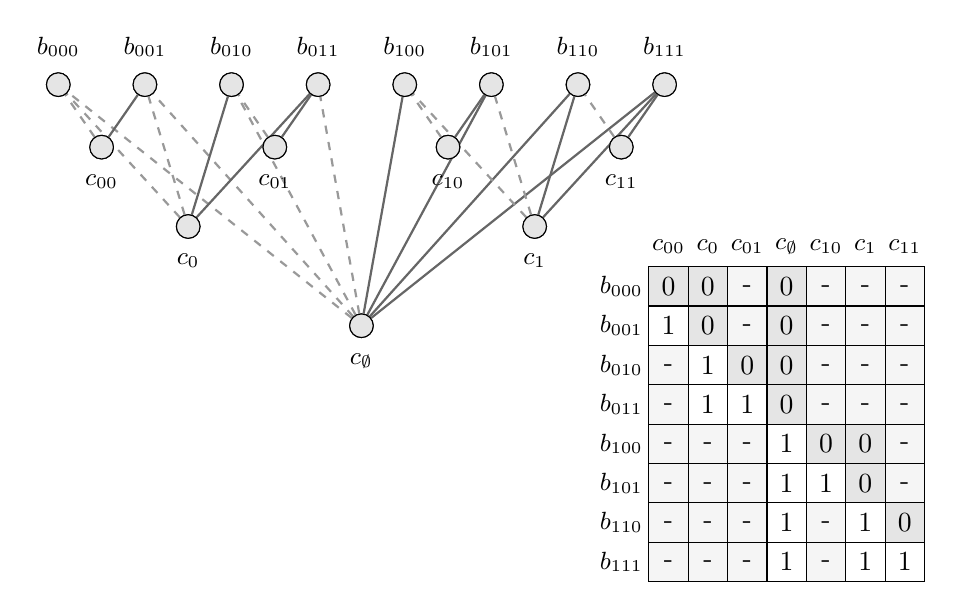
\begin{tikzpicture}[
        vertex/.style={circle, draw, fill=gray!20, minimum size=0.3cm, inner sep=1pt},
        label_c/.style={below=2pt, font=\small},
        label_b/.style={above=2pt, font=\small},
        solid edge/.style={draw, thick, black!60},
        dashed edge/.style={draw, dashed, thick, black!40},
        matrix cell/.style={draw, minimum size=0.5 cm, inner sep=0pt},
        matrix label/.style={font=\small, anchor=center}
    ]
	\node[vertex] (c_) at (4.4,0.0) {};
	\node[vertex] (c_0) at (2.2,1.26) {};
	\node[vertex] (c_1) at (6.6000000000000005,1.26) {};
	\node[vertex] (c_00) at (1.1,2.268) {};
	\node[vertex] (c_01) at (3.3000000000000003,2.268) {};
	\node[vertex] (c_10) at (5.5,2.268) {};
	\node[vertex] (c_11) at (7.700000000000001,2.268) {};
	\node[vertex] (b_000) at (0.55,3.0618) {};
	\node[vertex] (b_001) at (1.6500000000000001,3.0618) {};
	\node[vertex] (b_010) at (2.75,3.0618) {};
	\node[vertex] (b_011) at (3.8500000000000005,3.0618) {};
	\node[vertex] (b_100) at (4.95,3.0618) {};
	\node[vertex] (b_101) at (6.050000000000001,3.0618) {};
	\node[vertex] (b_110) at (7.15,3.0618) {};
	\node[vertex] (b_111) at (8.25,3.0618) {};
	\draw[dashed edge] (c_) -- (b_000);
	\draw[dashed edge] (c_) -- (b_001);
	\draw[dashed edge] (c_) -- (b_010);
	\draw[dashed edge] (c_) -- (b_011);
	\draw[solid edge] (c_) -- (b_100);
	\draw[solid edge] (c_) -- (b_101);
	\draw[solid edge] (c_) -- (b_110);
	\draw[solid edge] (c_) -- (b_111);
	\draw[dashed edge] (c_0) -- (b_000);
	\draw[dashed edge] (c_0) -- (b_001);
	\draw[solid edge] (c_0) -- (b_010);
	\draw[solid edge] (c_0) -- (b_011);
	\draw[dashed edge] (c_1) -- (b_100);
	\draw[dashed edge] (c_1) -- (b_101);
	\draw[solid edge] (c_1) -- (b_110);
	\draw[solid edge] (c_1) -- (b_111);
	\draw[dashed edge] (c_00) -- (b_000);
	\draw[solid edge] (c_00) -- (b_001);
	\draw[dashed edge] (c_01) -- (b_010);
	\draw[solid edge] (c_01) -- (b_011);
	\draw[dashed edge] (c_10) -- (b_100);
	\draw[solid edge] (c_10) -- (b_101);
	\draw[dashed edge] (c_11) -- (b_110);
	\draw[solid edge] (c_11) -- (b_111);
	\node[vertex] (c_) at (4.4,0.0) {};
	\node[vertex] (c_0) at (2.2,1.26) {};
	\node[vertex] (c_1) at (6.6000000000000005,1.26) {};
	\node[vertex] (c_00) at (1.1,2.268) {};
	\node[vertex] (c_01) at (3.3000000000000003,2.268) {};
	\node[vertex] (c_10) at (5.5,2.268) {};
	\node[vertex] (c_11) at (7.700000000000001,2.268) {};
	\node[vertex] (b_000) at (0.55,3.0618) {};
	\node[vertex] (b_001) at (1.6500000000000001,3.0618) {};
	\node[vertex] (b_010) at (2.75,3.0618) {};
	\node[vertex] (b_011) at (3.8500000000000005,3.0618) {};
	\node[vertex] (b_100) at (4.95,3.0618) {};
	\node[vertex] (b_101) at (6.050000000000001,3.0618) {};
	\node[vertex] (b_110) at (7.15,3.0618) {};
	\node[vertex] (b_111) at (8.25,3.0618) {};
	\node[label_c] at (c_.south) {$c_{\emptyset}$};
	\node[label_c] at (c_0.south) {$c_{0}$};
	\node[label_c] at (c_1.south) {$c_{1}$};
	\node[label_c] at (c_00.south) {$c_{00}$};
	\node[label_c] at (c_01.south) {$c_{01}$};
	\node[label_c] at (c_10.south) {$c_{10}$};
	\node[label_c] at (c_11.south) {$c_{11}$};
	\node[label_b] at (b_000.north) {$b_{000}$};
	\node[label_b] at (b_001.north) {$b_{001}$};
	\node[label_b] at (b_010.north) {$b_{010}$};
	\node[label_b] at (b_011.north) {$b_{011}$};
	\node[label_b] at (b_100.north) {$b_{100}$};
	\node[label_b] at (b_101.north) {$b_{101}$};
	\node[label_b] at (b_110.north) {$b_{110}$};
	\node[label_b] at (b_111.north) {$b_{111}$};

\begin{scope}[xshift=10.8 cm]
		\node[matrix cell, fill=gray!20] at (-2.5, 0.5) {0};
		\node[matrix cell] at (-2.5, 0.0) {1};
		\node[matrix cell, fill=gray!8] at (-2.5, -0.5) {-};
		\node[matrix cell, fill=gray!8] at (-2.5, -1.0) {-};
		\node[matrix cell, fill=gray!8] at (-2.5, -1.5) {-};
		\node[matrix cell, fill=gray!8] at (-2.5, -2.0) {-};
		\node[matrix cell, fill=gray!8] at (-2.5, -2.5) {-};
		\node[matrix cell, fill=gray!8] at (-2.5, -3.0) {-};
		\node[matrix cell, fill=gray!20] at (-2.0, 0.5) {0};
		\node[matrix cell, fill=gray!20] at (-2.0, 0.0) {0};
		\node[matrix cell] at (-2.0, -0.5) {1};
		\node[matrix cell] at (-2.0, -1.0) {1};
		\node[matrix cell, fill=gray!8] at (-2.0, -1.5) {-};
		\node[matrix cell, fill=gray!8] at (-2.0, -2.0) {-};
		\node[matrix cell, fill=gray!8] at (-2.0, -2.5) {-};
		\node[matrix cell, fill=gray!8] at (-2.0, -3.0) {-};
		\node[matrix cell, fill=gray!8] at (-1.5, 0.5) {-};
		\node[matrix cell, fill=gray!8] at (-1.5, 0.0) {-};
		\node[matrix cell, fill=gray!20] at (-1.5, -0.5) {0};
		\node[matrix cell] at (-1.5, -1.0) {1};
		\node[matrix cell, fill=gray!8] at (-1.5, -1.5) {-};
		\node[matrix cell, fill=gray!8] at (-1.5, -2.0) {-};
		\node[matrix cell, fill=gray!8] at (-1.5, -2.5) {-};
		\node[matrix cell, fill=gray!8] at (-1.5, -3.0) {-};
		\node[matrix cell, fill=gray!20] at (-1.0, 0.5) {0};
		\node[matrix cell, fill=gray!20] at (-1.0, 0.0) {0};
		\node[matrix cell, fill=gray!20] at (-1.0, -0.5) {0};
		\node[matrix cell, fill=gray!20] at (-1.0, -1.0) {0};
		\node[matrix cell] at (-1.0, -1.5) {1};
		\node[matrix cell] at (-1.0, -2.0) {1};
		\node[matrix cell] at (-1.0, -2.5) {1};
		\node[matrix cell] at (-1.0, -3.0) {1};
		\node[matrix cell, fill=gray!8] at (-0.5, 0.5) {-};
		\node[matrix cell, fill=gray!8] at (-0.5, 0.0) {-};
		\node[matrix cell, fill=gray!8] at (-0.5, -0.5) {-};
		\node[matrix cell, fill=gray!8] at (-0.5, -1.0) {-};
		\node[matrix cell, fill=gray!20] at (-0.5, -1.5) {0};
		\node[matrix cell] at (-0.5, -2.0) {1};
		\node[matrix cell, fill=gray!8] at (-0.5, -2.5) {-};
		\node[matrix cell, fill=gray!8] at (-0.5, -3.0) {-};
		\node[matrix cell, fill=gray!8] at (0.0, 0.5) {-};
		\node[matrix cell, fill=gray!8] at (0.0, 0.0) {-};
		\node[matrix cell, fill=gray!8] at (0.0, -0.5) {-};
		\node[matrix cell, fill=gray!8] at (0.0, -1.0) {-};
		\node[matrix cell, fill=gray!20] at (0.0, -1.5) {0};
		\node[matrix cell, fill=gray!20] at (0.0, -2.0) {0};
		\node[matrix cell] at (0.0, -2.5) {1};
		\node[matrix cell] at (0.0, -3.0) {1};
		\node[matrix cell, fill=gray!8] at (0.5, 0.5) {-};
		\node[matrix cell, fill=gray!8] at (0.5, 0.0) {-};
		\node[matrix cell, fill=gray!8] at (0.5, -0.5) {-};
		\node[matrix cell, fill=gray!8] at (0.5, -1.0) {-};
		\node[matrix cell, fill=gray!8] at (0.5, -1.5) {-};
		\node[matrix cell, fill=gray!8] at (0.5, -2.0) {-};
		\node[matrix cell, fill=gray!20] at (0.5, -2.5) {0};
		\node[matrix cell] at (0.5, -3.0) {1};
		\node[matrix label] at (-3.1, 0.5) {$b_{000}$};
		\node[matrix label] at (-3.1, 0.0) {$b_{001}$};
		\node[matrix label] at (-3.1, -0.5) {$b_{010}$};
		\node[matrix label] at (-3.1, -1.0) {$b_{011}$};
		\node[matrix label] at (-3.1, -1.5) {$b_{100}$};
		\node[matrix label] at (-3.1, -2.0) {$b_{101}$};
		\node[matrix label] at (-3.1, -2.5) {$b_{110}$};
		\node[matrix label] at (-3.1, -3.0) {$b_{111}$};
		\node[matrix label] at (-2.5, 1) {$c_{00}$};
		\node[matrix label] at (-2.0, 1) {$c_{0}$};
		\node[matrix label] at (-1.5, 1) {$c_{01}$};
		\node[matrix label] at (-1.0, 1) {$c_{\emptyset}$};
		\node[matrix label] at (-0.5, 1) {$c_{10}$};
		\node[matrix label] at (0.0, 1) {$c_{1}$};
		\node[matrix label] at (0.5, 1) {$c_{11}$};
    \end{scope}

    \end{tikzpicture}
    
    \label{fig:k_tree}
\end{figure}

\end{frame}

% relation between k-trees and non-k-order property: k-tree in 2^k-order
\begin{frame}{Sketch of the Proof of the Stable Regularity Lemma}
    \input{pictures/half-graph_implies_k-tree_presentation}
\end{frame}

% relation between k-trees and non-k-order property: 2^k-order in k-tree
\begin{frame}{Sketch of the Proof of the Stable Regularity Lemma}
    \begin{theorem}[Lemma 6.7.9 in~\cite{model_theory}] \label{thm:tree_implies_order}
        \visible<1-> {
            If a graph $G$ has the $2^{k_{**}}$-order property, then the tree bound of $G$ is at least $k_{**} + 1$.
        }

        \visible<2-> {
            On the other hand, if a graph $G$ has tree bound at least $k_{**} = 2^{k_*+1}-1$, then it has the $k_*$-order
            property.
        }
    \end{theorem}
\end{frame}

% existence of excellent sets
\begin{frame}{Sketch of the Proof of the Stable Regularity Lemma}
    % 1
    \begin{lemma}[Existence of excellent subsets,~\cite{regularity_lemmas_for_stable_graphs}]<1-> \label{lem:existance_of_excellent_subsets}
        Let $G$ be a finite graph with the non-$k_{*}$-order property.
        Let $\zeta \leq \frac{1}{2^{k_{**}}}$, $\epsilon \in \parround{0, \frac{1}{2}}$.
        Then, for every $A \subseteq G$ with $|A| \geq \frac{1}{\epsilon^{k_{**}}}$ there exists an $(\epsilon, \zeta)$-excellent
        subset $A' \subseteq A$ such that $|A'| \geq \epsilon^{k_{**}-1} |A|$.
    \end{lemma}

    % 2
    \visible<2-> {
        TO DO
    }
\end{frame}

% existence of excellent sets: proof sketch
\begin{frame}{Sketch of the Proof of the Stable Regularity Lemma}
    \begin{figure}
    \centering
    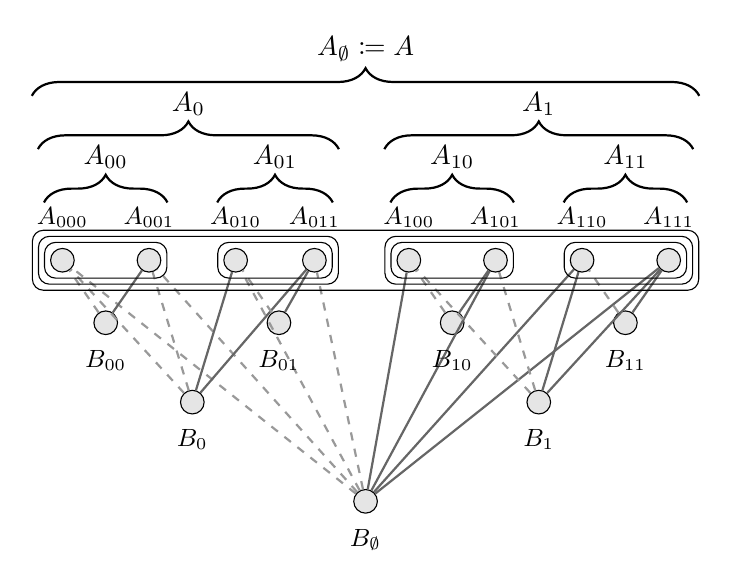
\begin{tikzpicture}[
        vertex/.style={circle, draw, fill=gray!20, minimum size=0.3cm, inner sep=1pt},
        label_c/.style={below=2pt, font=\small},
        label_b/.style={above=4pt, font=\small},
        solid edge/.style={draw, thick, black!60},
        dashed edge/.style={draw, dashed, thick, black!40},
    ]
    \uncover<7-> {
        \node[vertex] (b_000) at (0.55,3.0618) {};
        \node[vertex] (b_001) at (1.6500000000000001,3.0618) {};
        \node[vertex] (b_010) at (2.75,3.0618) {};
        \node[vertex] (b_011) at (3.7500000000000005,3.0618) {};
        \node[vertex] (b_100) at (4.95,3.0618) {};
        \node[vertex] (b_101) at (6.050000000000001,3.0618) {};
        \node[vertex] (b_110) at (7.15,3.0618) {};
        \node[vertex] (b_111) at (8.25,3.0618) {};
    }
    \uncover<2-> {
        \node[vertex] (c_) at (4.4,0.0) {};
        \node[label_c] at (c_.south) {$B_{\emptyset}$};
    }
    \uncover<7-> {
        \node[label_b] at (b_000.north) {$A_{000}$};
        \node[label_b] at (b_001.north) {$A_{001}$};
        \node[label_b] at (b_010.north) {$A_{010}$};
        \node[label_b] at (b_011.north) {$A_{011}$};
        \node[label_b] at (b_100.north) {$A_{100}$};
        \node[label_b] at (b_101.north) {$A_{101}$};
        \node[label_b] at (b_110.north) {$A_{110}$};
        \node[label_b] at (b_111.north) {$A_{111}$};
    }
    \uncover<4-> {
        \node[vertex] (c_0) at (2.2,1.26) {};
        \node[vertex] (c_1) at (6.6000000000000005,1.26) {};
        \node[label_c] at (c_0.south) {$B_{0}$};
        \node[label_c] at (c_1.south) {$B_{1}$};
    }
    \uncover<6-> {
        \node[vertex] (c_00) at (1.1,2.268) {};
        \node[vertex] (c_01) at (3.3000000000000003,2.268) {};
        \node[vertex] (c_10) at (5.5,2.268) {};
        \node[vertex] (c_11) at (7.700000000000001,2.268) {};
    }
    \uncover<3-> {
        \draw[dashed edge] (c_) -- (b_000);
        \draw[dashed edge] (c_) -- (b_001);
        \draw[dashed edge] (c_) -- (b_010);
        \draw[dashed edge] (c_) -- (b_011);
        \draw[solid edge] (c_) -- (b_100);
        \draw[solid edge] (c_) -- (b_101);
        \draw[solid edge] (c_) -- (b_110);
        \draw[solid edge] (c_) -- (b_111);
    }
    \uncover<5-> {
        \draw[dashed edge] (c_0) -- (b_000);
        \draw[dashed edge] (c_0) -- (b_001);
        \draw[solid edge] (c_0) -- (b_010);
        \draw[solid edge] (c_0) -- (b_011);
        \draw[dashed edge] (c_1) -- (b_100);
        \draw[dashed edge] (c_1) -- (b_101);
        \draw[solid edge] (c_1) -- (b_110);
        \draw[solid edge] (c_1) -- (b_111);
    }
    \uncover<7-> {
        \draw[dashed edge] (c_00) -- (b_000);
        \draw[solid edge] (c_00) -- (b_001);
        \draw[dashed edge] (c_01) -- (b_010);
        \draw[solid edge] (c_01) -- (b_011);
        \draw[dashed edge] (c_10) -- (b_100);
        \draw[solid edge] (c_10) -- (b_101);
        \draw[dashed edge] (c_11) -- (b_110);
        \draw[solid edge] (c_11) -- (b_111);
    }
    \uncover<6-> {
        \node[label_c] at (c_00.south) {$B_{00}$};
        \node[label_c] at (c_01.south) {$B_{01}$};
        \node[label_c] at (c_10.south) {$B_{10}$};
        \node[label_c] at (c_11.south) {$B_{11}$};
    }
    \uncover<5-> {
        \node[draw, rounded corners, fit=(b_000) (b_001), inner sep=.7mm] (box00) {};
        \draw [decorate, thick, decoration={brace, amplitude=10pt, mirror, raise=5mm}] (box00.north east) -- (box00.north west)
            node [above=8mm, midway] {$A_{00}$};
        \node[draw, rounded corners, fit=(b_010) (b_011), inner sep=.7mm] (box01) {};
        \draw [decorate, thick, decoration={brace, amplitude=10pt, mirror, raise=5mm}] (box01.north east) -- (box01.north west)
            node [above=8mm, midway] {$A_{01}$};
        \node[draw, rounded corners, fit=(b_100) (b_101), inner sep=.7mm] (box10) {};
        \draw [decorate, thick, decoration={brace, amplitude=10pt, mirror, raise=5mm}] (box10.north east) -- (box10.north west)
            node [above=8mm, midway] {$A_{10}$};
        \node[draw, rounded corners, fit=(b_110) (b_111), inner sep=.7mm] (box11) {};
        \draw [decorate, thick, decoration={brace, amplitude=10pt, mirror, raise=5mm}] (box11.north east) -- (box11.north west)
            node [above=8mm, midway] {$A_{11}$};
    }
    \uncover<3-> {
        \node[draw, rounded corners, fit=(box00) (box01), inner sep=.7mm] (box0) {};
        \draw [decorate, thick, decoration={brace, amplitude=10pt, mirror, raise=11mm}] (box0.north east) -- (box0.north west)
            node [above=14mm, midway] {$A_{0}$};
        \node[draw, rounded corners, fit=(box10) (box11), inner sep=.7mm] (box1) {};
        \draw [decorate, thick, decoration={brace, amplitude=10pt, mirror, raise=11mm}] (box1.north east) -- (box1.north west)
            node [above=14mm, midway] {$A_{1}$};
    }
    \uncover<1-> {
        \node[draw, rounded corners, fit=(box0) (box1), inner sep=.7mm] (box) {};
        \draw [decorate, thick, decoration={brace, amplitude=10pt, mirror, raise=17mm}] (box.north east) -- (box.north west)
            node [above=20mm, midway] {$A_\emptyset \coloneqq A$};
    }
    \end{tikzpicture}
    
    \label{fig:k_tree_for_existence}
\end{figure}

\end{frame}

% we can actually ensure size is in a given sequence of sizes with not much extra work
\begin{frame}{Sketch of the Proof of the Stable Regularity Lemma}
    \begin{lemma}[Existence of excellent subsets,~\cite{regularity_lemmas_for_stable_graphs}]
        Let $G$ be a finite graph with the non-$k_{*}$-order property.
        Let $\zeta < \frac{1}{2^{k_{**}}}$, $\epsilon \in \parround{0, \frac{1}{2}}$.
        Let $\Partriangle{m_\ell \mid \ell \in \parcurly{0, \dots, k_{**}}}$ be a decreasing sequence of natural numbers such that
        $\epsilon m_{\ell} \geq m_{\ell+1}$ for all $\ell \in \parcurly{0, \dots, k_{**}-1}$ and $m_{k_{**}} \geq 1$.
        Then, for every $A \subseteq G$ with $|A| \geq m_0$ there exists
        $\parround{\frac{m_{\ell+1}}{m_{\ell}}, \zeta}$-excellent subset $A' \subseteq A$ such that $|A'| = m_\ell$ for
        some $\ell \in \parcurly{0, \dots, k_{**}-1}$.
    \end{lemma}
\end{frame}

% building uneven partition
\begin{frame}{Sketch of the Proof of the Stable Regularity Lemma}
    \begin{lemma} \label{lem:existance_of_excellent_partition}
        Let $G$ be a finite graph with the non-$k_{*}$-order property.
        Let $\epsilon \in \parround{0, \frac{1}{2}}$ and $\epsilon' \leq \frac{1}{2^{k_{**}}}$.
        Let $A \subseteq G$ such that $|A| = n \geq m_0$.
        Let $\Partriangle{m_\ell \mid \ell \in \parcurly{0, \dots, k_{**}}}$ be a decreasing sequence of natural numbers such that
        $\epsilon m_{\ell} \geq m_{\ell+1}$ for all $\ell \in \parcurly{0, \dots, k_{**}-1}$ and $m_{k_{**}} \geq 1$.
        Denote $m_* \coloneqq m_0$ and $m_{**} \coloneqq m_{k_{**}}$.
        Then, there is a partition $\overline{A} = \Partriangle{A_j \mid j \in \parcurly{1, \dots, j(*)}}$ with remainder
        $B = A \setminus \bigcup_{j < j(*)} A_j$ such that:
        \begin{enumerate}
            \item For all $j \in \parcurly{1, \dots, j(*)}$, $|A_j| \in \Partriangle{m_\ell \mid \ell \in \parcurly{0, \dots, k_{**}-1}}$.
            \item For all $i \neq j \in \parcurly{1, \dots, j(*)}$, $A_i \cap A_j = \emptyset$.
            \item For all $j \in \parcurly{1, \dots, j(*)}$, $A_j$ is $\parround{\epsilon, \epsilon'}$-excellent.
            \item $|B| < m_*$.
        \end{enumerate}
    \end{lemma}
\end{frame}

% refining to an equitable partition
\begin{frame}{Sketch of the Proof of the Stable Regularity Lemma}
    \visible<1-> {
        \textbf{Question:} Are subsets of excellent sets still excellent?
    }

    \visible<2-> {
        \textbf{Answer:} With high probability, yes, but with a small loss in excellence.
    }

    \begin{lemma}<3->
        Let $G$ be a finite graph with the non-$k_{*}$-order property.
        Then, for every $\epsilon \in \parround{0, \frac{1}{2}}$,
        $\zeta \in \parround{0, \frac{1}{2} - \epsilon}$, $\xi \in \parround{0, 1}$ and
        $m \geq \frac{1}{\zeta^2}\parround{k_* \log{\frac{1}{\zeta^2}k_*} - \log{\xi}}$,
        if $A \subseteq G$ is an $\epsilon$-good subset of size $n \geq m$,
        then a subset $A' \subseteq A$ of size $m$, sampled uniformly at random, is $(\epsilon + \zeta)$-good with probability $1-\xi$.
    \end{lemma}

    \begin{lemma}<4->
        Let $G$ be a finite graph with the non-$k_{*}$-order property.
        Then, for every $\zeta \in \parcurly{0, \frac{1}{2}}$ and $\zeta' < \zeta$, there is
        $\epsilon_1 = \epsilon_1(\zeta, \zeta')$ such that for every $\epsilon < \epsilon' \leq \epsilon_1$, if
        \begin{itemize}
            \item $A \subseteq G$ is $\parround{\epsilon, \epsilon'}$-excellent and
            \item $A' \subseteq A$ is $\parround{\epsilon + \zeta'}$-good,
        \end{itemize}
        then, $A'$ is $\parround{\epsilon + \zeta, \epsilon'}$-excellent.
    \end{lemma}
\end{frame}

% distribute remainder evenly across parts
\begin{frame}{Sketch of the Proof of the Stable Regularity Lemma}
\end{frame}

% excellence implies regularity and homogeneity
\begin{frame}{Sketch of the Proof of the Stable Regularity Lemma}
\end{frame}

% final result
\begin{frame}{Sketch of the Proof of the Stable Regularity Lemma}
\end{frame}

% ---

% what is property testing and H-freeness
\begin{frame}{Property Testing of $H$-freeness in Stable Graphs}
\end{frame}

% previous results with SzRL
\begin{frame}{Property Testing of $H$-freeness in Stable Graphs}
\end{frame}

% unavoidability implies abundance
\begin{frame}{Property Testing of $H$-freeness in Stable Graphs}
\end{frame}

% the algorithm
\begin{frame}{Property Testing of $H$-freeness in Stable Graphs}
\end{frame}

% ---

% limitations of the algorithm
\begin{frame}{Conclusion and Future Work}
\end{frame}

% lines of research with Lluis
\begin{frame}{Conclusion and Future Work}
\end{frame}

\begin{frame}{Conclusion and Future Work}
\end{frame}

\begin{frame}{Conclusion and Future Work}
\end{frame}

% ---

% Thanks
\begin{frame}
    \centering
    \Huge{\textbf{Thank you!}}
    \vspace{1em}

    \Large{You can now rate the presentation.
    Was it \emph{good}, \emph{excellent} or \emph{exceptional}?}
\end{frame}

\end{document}